\documentclass[a4paper,10pt]{scrreprt}

\usepackage[ngerman]{babel}
\usepackage{graphicx}
\usepackage[utf8]{inputenc}
\usepackage{listings}
\usepackage{scrhack}
\usepackage{hyperref}
\usepackage[
  acronym,
  nomain,
  toc,
  xindy
]{glossaries}

% Listings konfigurieren
\lstset{
  aboveskip = \floatsep,
  captionpos = b,
  basicstyle = \ttfamily\small,
  breaklines = true,
  frame = single,
  numbers = left,
  numberstyle = \tiny,
  showstringspaces = false
}

\makeglossaries

\title{AntScout-Dokumentation}
\author{Alexander Bertram}

\begin{document}

\maketitle

\newacronym{osm}{OSM}{\textit{OpenStreetMap}}
\newacronym{url}{URL}{Uniform Resource Locator}


\printglossary[
  title = Abkürzungsverzeichnis,
  toctitle = Abkürzungsverzeichnis
]

\chapter{Typografische Konventionen}
\label{chap:typografische-konventionen}

Konsolen-Kommandos, URLs oder Quellcode-Ausschnitte im Fließtext werden in einer \texttt{Nicht-Proportionalschrift} dargestellt.

\chapter{Allgemeine Problemstellung}
\label{chap:allgemeine-problemstellung}

Im Rahmen des Master-Projektes und der -Thesis soll eine Anwendung erstellt werden, in der der Ameisen-Algorithmus \textit{AntNet} auf realen Strassen-Karten für das dynamische Routing implementiert wird.
Die Daten werden von \textit{OpenStreetMap} abgerufen und in einen Graphen umgewandelt, auf dem \textit{AntNet} operieren kann.
Die Erstellung der Anwendung ist in zwei Schritte unterteilt:

\begin{enumerate}
  \item Abruf und Aufbereitung der Daten
  \item \textit{AntNet}-Implementierung
\end{enumerate}

Der erste Schritt ist das Ziel des Master-Projektes und der zweite das Ziel der Master-Thesis.

\chapter{Benutzerhandbuch}
\label{chap:benutzerhandbuch}

\section{Ablaufbedingungen}
\label{sec:ablaufbedingungen}

\section{Installation}
\label{sec:installation}

\textit{AntScout} benötigt keine Installation.
Das Archiv muss lediglich auf die lokale Festplatte extrahiert werden.
Dabei wird der Ordner ``AntScout'' erstellt, der alles beinhaltet, was für den Start der Anwendung nötig ist.

\section{Programmstart}
\label{sec:programmstart}

\subsection{Voraussetzungen}
\label{sec:voraussetzungen}

\begin{itemize}
  \item Eine bestehende Internet-Verbindung.
  \item Eine möglichst aktuelle Java-Version von Oracle.
  \item Der lokale Port \texttt{8080} darf nicht durch eine bereits laufende Anwendung blockiert sein.
\end{itemize}

\subsection{Start}
\label{sec:programmstart-start}

\begin{enumerate}
  \item Konsole (auch Eingabeaufforderung oder Kommandozeile genannt) öffnen
  \item In das erstellte Verzeichnis ``AntScout'' wechseln
  \item \texttt{sbt}
  \item \texttt{container:start}
  \item \texttt{http://localhost:8080} oder \texttt{http://127.0.0.1:8080} im Browser aufrufen
\end{enumerate}

\subsection{Hinweise}
\label{sec:programmstart-hinweise}

\begin{itemize}
  \item Nach dem Start von \texttt{sbt} werden alle benötigten Bibliotheken heruntergeladen.
    Je nach Internet-Verbindung kann dieser Vorgang mehrere Minuten dauern.
  \item Nach der Eingabe von \texttt{container:start} werden die benötigten Karten heruntergeladen und vorverarbeitet.
    Dieser Vorgang kann auch je nach Internet-Verbindung und Computer-Leistung mehrere Minuten dauern.
  \item Es sollte nach Möglichkeit ein möglichst moderner Browser, der HTML5 unterstützt, verwendet werden.
\end{itemize}

\section{Programmende}
\label{sec:programmende}

\begin{enumerate}
  \item \texttt{container:stop}
  \item \texttt{exit}
\end{enumerate}

oder einfach die Konsole schliessen.

\section{Bedienungsanleitung}
\label{sec:bedienungsanleitung}

\subsection{Front-End}
\label{sec:front-end}

Nach dem Aufruf \texttt{http://localhost:8080} im Browser öffnet sich die Start-Seite.
Ein Screenshot dieser Seite ist in der Abbildung \ref{fig:start-seite} zu sehen.

\begin{figure}[htbp]
  \centering
  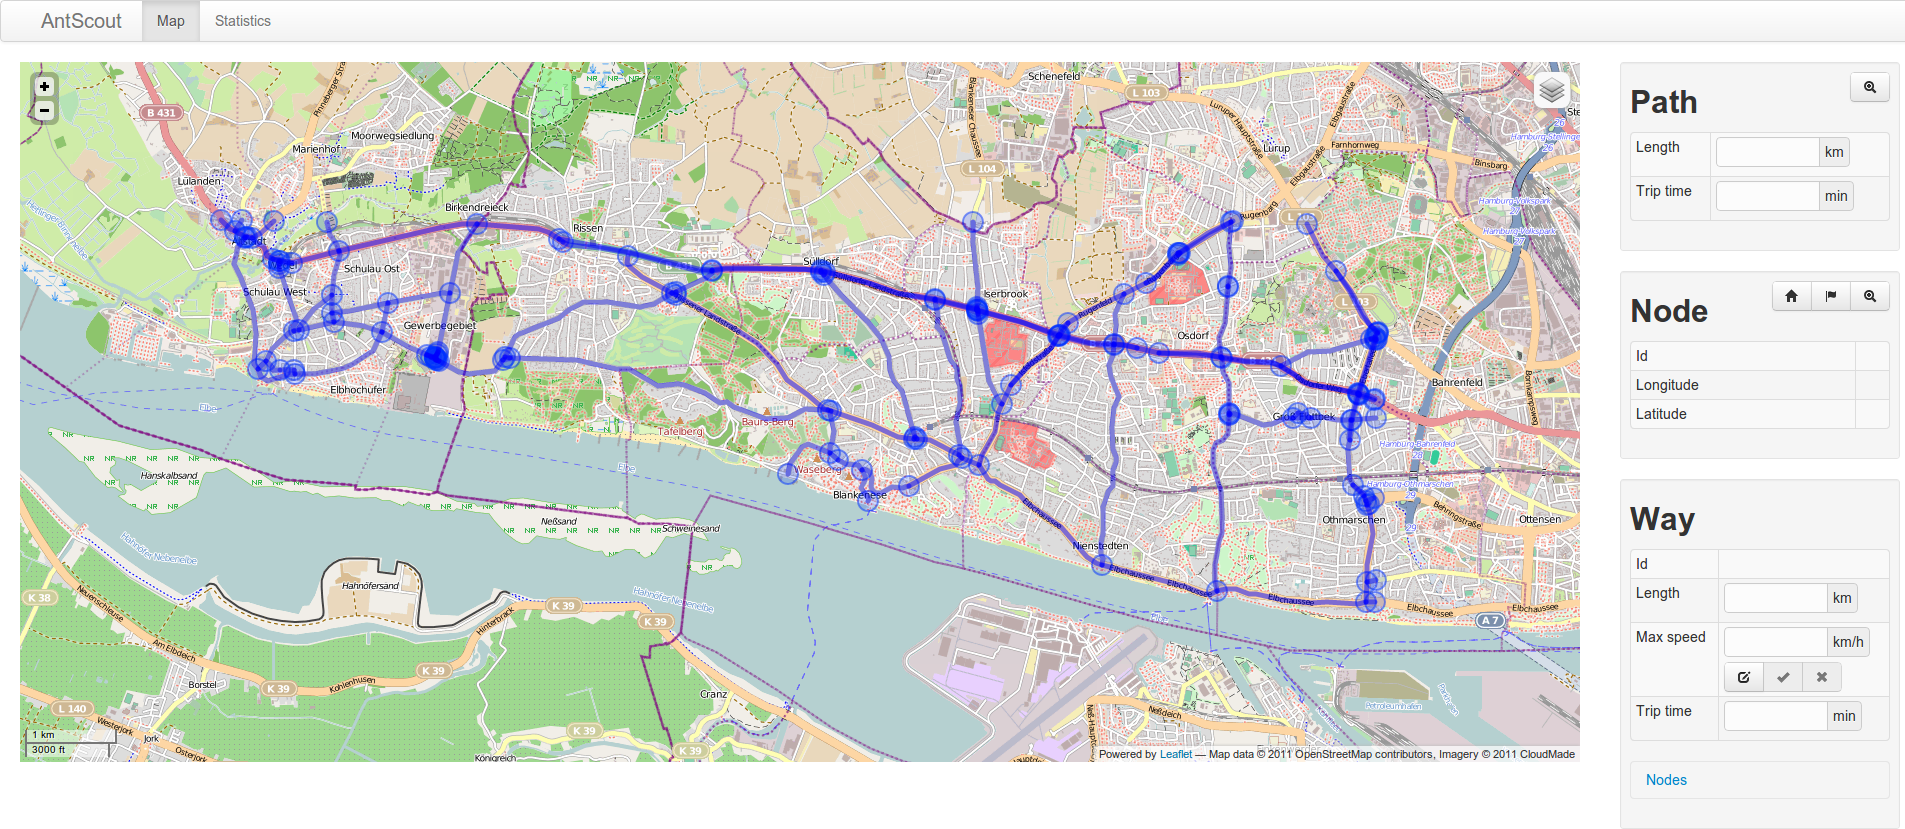
\includegraphics[width=\textwidth]{Bilder/Start-Seite.png}
  \caption{Start-Seite}
  \label{fig:start-seite}
\end{figure}

Die Seite ist in drei Bereiche unterteilt:

\subsubsection{Menü}
\label{sec:menue}

Die obere Leiste stellt das Menü dar.
Hier kann zwischen der Karten- und der Statistiken-Ansicht (siehe Abschnitt \ref{sec:statistiken}) umgeschaltet werden.

\subsubsection{Karte}
\label{sec:karte}

Die Karte nimmt den größten Platz der Seite ein.
Hier sind die Kreuzungen - nachfolgend Knoten genannt - zu sehen, zwischen denen navigiert werden kann und die Wege, die die Knoten verbinden.
Jeder Knoten und jeder Weg kann durch einen Maus-Klick markiert werden.
Dieser wird dann optisch hervorgehoben.

\subsubsection{Informationen}
\label{sec:informationen}

Der Informationen-Bereich auf der rechten Seite ist in drei weitere Bereiche unterteilt:

\paragraph{Pfad}
\label{sec:pfad}

Wenn ein Pfad gefunden wurde, werden hier die Länge und die Passier-Zeit angezeigt (siehe Abbildung \ref{fig:pfad-informationen}).
Mit dem Button rechts oben können weitere Informationen eingeblendet werden.

\begin{figure}[htbp]
  \centering
  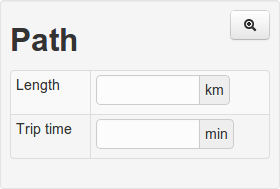
\includegraphics[width=0.3\textwidth]{Bilder/Pfad-Informationen.png}
  \caption{Pfad-Informationen}
  \label{fig:pfad-informationen}
\end{figure}

\paragraph{Knoten}
\label{sec:knoten}

Nach der Markierung eines Knotens werden in diesem Bereich die Knoten-Daten eingetragen.
Es handelt sich um die Id und die geographischen Daten, die direkt aus \gls{osm} übernommen werden (siehe Abbildung \ref{fig:knoten-informationen}).

\begin{figure}[htbp]
  \centering
  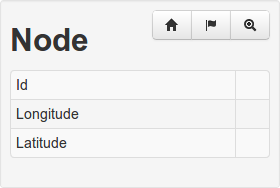
\includegraphics[width=0.3\textwidth]{Bilder/Knoten-Informationen.png}
  \caption{Knoten-Informationen}
  \label{fig:knoten-informationen}
\end{figure}

Die drei Buttons rechts oben im Knoten-Informationen-Bereich (siehe Abbildung \ref{fig:knoten-buttons}) führen verschiedene Aktionen aus.
Mit dem linken kann die aktuell selektierte Kreuzung als Start und mit dem mittleren als Ziel gesetzt werden.
Ein als Start oder Ziel gesetzter Knoten wird mit einem entsprechenden Marker versehen (siehe Abbildungen \ref{fig:start-knoten} und \ref{fig:ziel-knoten}).
Mit dem rechten Button können weitere Informationen über die aktuell selektierte Knoten-Konstellation eingeblendet werden.

\begin{figure}[htbp]
  \centering
  
\includegraphics[width=0.15\textwidth]{Bilder/Knoten-Buttons.png}
  \caption{Knoten-Buttons}
  \label{fig:knoten-buttons}
\end{figure}

\begin{figure}[htbp]
  \centering
  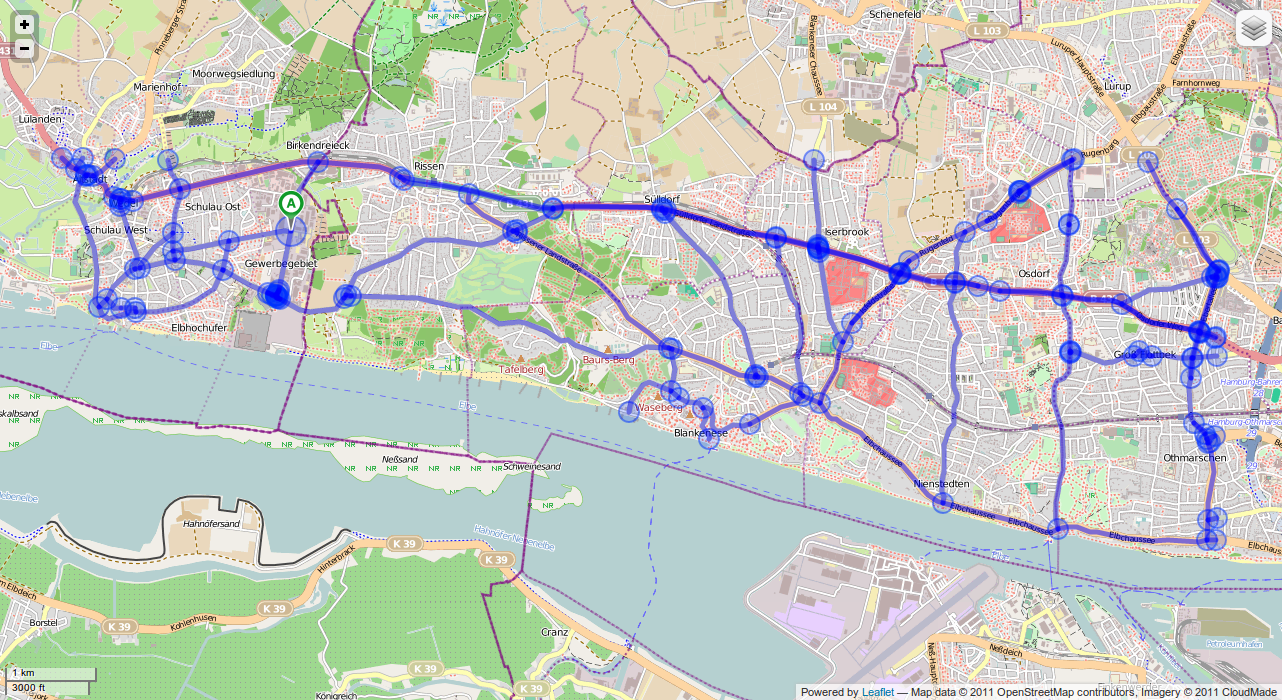
\includegraphics[width=\textwidth]{Bilder/Start-Knoten.png}
  \caption{Start-Knoten}
  \label{fig:start-knoten}
\end{figure}

\begin{figure}[htbp]
  \centering
  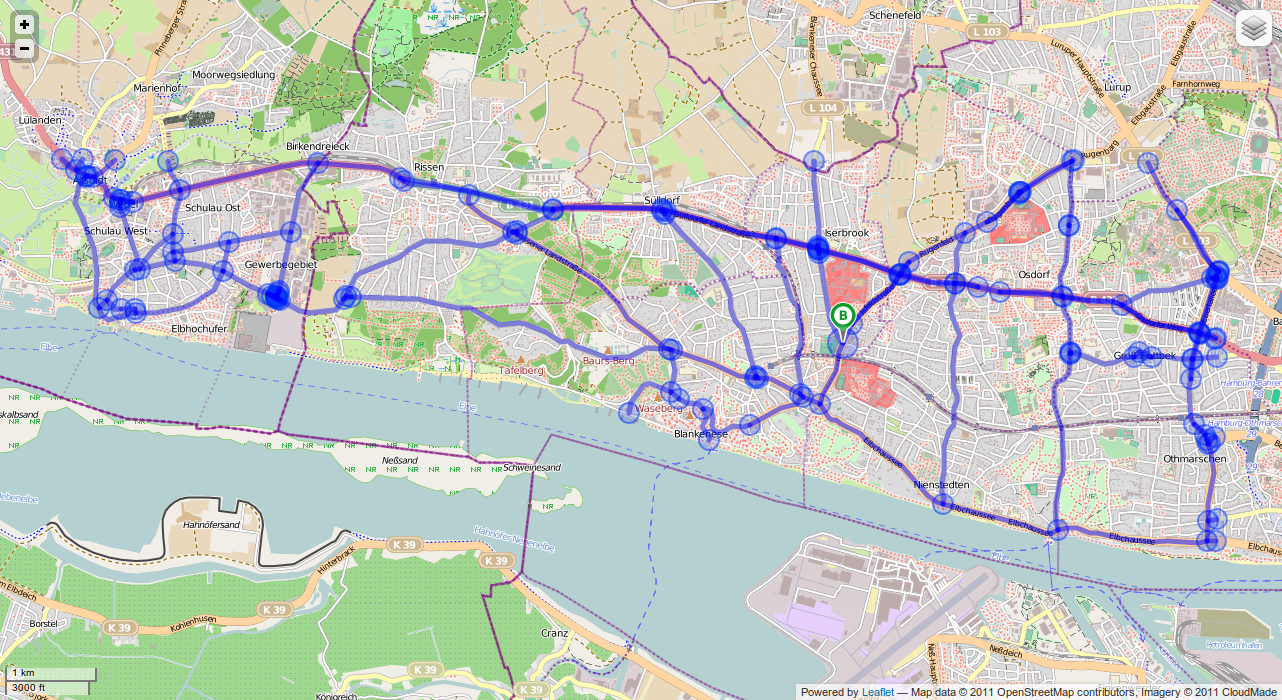
\includegraphics[width=\textwidth]{Bilder/Ziel-Knoten.png}
  \caption{Ziel-Knoten}
  \label{fig:ziel-knoten}
\end{figure}

\paragraph{Weg}
\label{sec:weg}

Hier werden die Daten eines selektierten Weges angezeigt.
Neben einer Weg-Id werden hier die Länge, die maximale Geschwindigkeit und die Knoten angezeigt, aus denen der Weg besteht.

\subsubsection{Statistiken}
\label{sec:statistiken}

\subsection{Konfiguration}
\label{sec:konfiguration}

\textbf{Achtung!}
Hier sollten nur fortgeschrittene Benutzer etwas ändern.
Es besteht die Gefahr einer ungültigen Konfiguration.
Dann gibt \textit{AntScout} beim Starten eine Fehlermeldung aus und startet nicht mehr richtig.

Im Verzeichnis \texttt{AntScout/src/main/resources} befindet sich die Datei \texttt{reference.conf}.
Dort sind die Einstellungen für \textit{AntScout} zu finden.
Die Datei ist eine Text-Datei und kann mit einem Text-Editor bearbeitet werden.

Die Konfiguration ist in mehrere Ebenen unterteilt, wobei \texttt{ant-scout} die oberste Ebene darstellt.
Jede ebene ist in geschweifte Klammern eingeschlossen.

Jeder Parameter ist durch einen Namen und einen Wert definiert.

\begin{lstlisting}
name = wert
\end{lstlisting}

Jede Änderung der Konfiguration wird erst nach einem Neustart der Applikation wirksam.

\subsubsection{Karte}
\label{sec:konfiguration-karte}

Der Parameter \texttt{map} steuert, welche Karte verwendet werden soll.
Es sind mehrere Karten in verschiedenen Größen vordefiniert.
Die Zeile, die die aktuell verwendete Karte enthält, ist die einzige, die nicht mit einem \#-Zeichen beginnt.
Dieser Zeile muss ein \#-Zeichen vorangestellt werden, damit sie nicht mehr verwendet wird.
Vor der Zeile, die die gewünschte Karte enthält, muss das \#-Zeichen entfernt werden.

\begin{lstlisting}
# Karte, die verwendet werden soll.
# 104 Knoten, 99 Quellen und 100 Ziele
# map = maps/Bahrenfeld-Gross-Flottbek-Othmarschen-Ottensen.osm
# 85 Knoten, 83 Quellen und 83 Ziele
# map = maps/Blankenese-Wedel.osm
# 47 Knoten, 43 Quellen und 45 Ziele
map = maps/Altona-50-Knoten.osm
# 14 Knoten, 12 Quellen und Ziele
# map = maps/Altona-Kreis.osm
# 142 Knoten, 138 Quellen und Ziele
# map = maps/Altona-Wedel.osm
# 57 Knoten, 57 Quellen und 56 Ziele
# map = maps/Wedel.osm
\end{lstlisting}


\section{Fehlermeldungen}
\label{sec:fehlermeldungen}

\section{Wiederanlaufbedingungen}
\label{sec:wiederanlaufbedingungen}

\chapter{Programmierhandbuch}
\label{chap:Programmierhandbuch}

\section{Entwicklungskonfiguration}
\label{sec:entwicklungskonfiguration}

\section{Problemanalyse und Realisation}
\label{sec:problemanalyse-und-realisation}

\section{Beschreibung grundlegender Datenstrukturen}
\label{sec:beschreibung-grundlegender-datenstrukturen}

\section{Programmorganisation}
\label{sec:programmorganisation}

\section{Programmtest}
\label{sec:programmtest}

\end{document}
